The Online Shoppers Purchasing Prediction dataset fits somewhere in between the others as it has a low to medium amount of features and its sample size is on the medium to high spectrum. It also complements the Breast Cancer dataset as it is also a binary classification task. Another reason why  this dataset has been chosen, is that is a lot closer to real world applications than some other posed Machine Learning questions. From a entrepreneurial standpoint it is very interesting for business processes as it can aid in ameliorating other internal processes. With it one can facilitate answering questions such as ''Will this person buy something?'' and ''How can we change our internal processes, based on the important attributes we identified, to increase the percentage of people buying things?''. We first take a general look on the different attributes and try to find the most important features by analysing the data. Afterwards we try out the above mentioned classifiers with a few different parameters to find the right settings based on this dataset. A final summary will be given by comparing the best parameters in combination with Preprocessing vs No-Preprocessing, Holdout vs Cross Validation and taking a look at a few different performance metrics.

\subsection{Characteristics}

\begin{itemize}
\item Missing values in the original dataset
\item Binary Target Class Revenue
\item 18 attributes (10 numerical, 8 categorical)
\item Nominal attributes (Browser, OS, Region, ...)
\item Interval attributes (Bounce Rate, Exit Rate, ...)
\item Ratio attributes (Informational Duration, ProductRelated Duration, ..)
\item 12330 samples
\end{itemize}

\subsection{General Preprocessing} \label{GenPrepro}
The \textbf{original} dataset contained 14 missing values which could easily be resolved by just removing the affected rows. Another thing that could be done, would be to replace the ratio and interval attributes with the mean and the ordinal and the categorical attributes with the median. On the UCI Machine Learning Repository we were able to find a version of this dataset which contained no missing values, hence no further action was needed. \\
\newline
As there are 8 categorical values these need to be encoded to be available for our Classifiers. Instead of using Label Encoding, where higher values could be biased, we used One Hot Encoding. This added about 40 features to our already existing ones.

\subsection{Characteristics of Target Value}
While accuracy is a great measure for classification problems when one has symmetric datasets (amount of false positves and false negatives is approximately the same), it is not optimal for our model.
As can be seen in \secref{fig:rev_box} only 15.5\% (1908) were positive class samples that ended with shopping and the rest (10422) did not end with shopping. It is more important to not falsely identify Buyers as Non-Buyers. For example we would rather focus on more people than necessary instead of potentially losing profit and customers. Due to this we chose Recall as our primary performance metric when optimizing the different Classifiers as there is a high cost of False Negatives and our data is skewed.
\image{onlineshop/plots/revenue_boxplot.png}{Target Class Distribution Online Shopping Predictions Revenue}{\label{fig:rev_box}}

\subsection{Feature Selection}
% Heatmap Correlation
Now having 57 attributes, it is important to remove features and thus random noise which could lead to overfitting to the training data. Reducing the dimensions also allows us to reduce training time and thus lets us train with more different parameters. Looking at the correlation matrix in \secref{fig:heat} one can see features that are correlated such as PageValues, ExitRates, ProductRelated,ProductRelated Duration BounceRates, etc.  
\image{onlineshop/plots/heatmap.png}{Heatmap of the different attributes of the Online Shopping Prediction dataset}{\label{fig:heat}} \\
\newline
Using Scikitlearn's SelectKBest and RandomForestClassifier we analysed the features, correlating with the Revenue target, more in depth. The top 10 correlated features, with their respective scores, found through SelectKBest are found in \secref{fig:feat_rfc} and Table \secref{tab:feat_sel}. \\

\begin{figure}
\begin{floatrow}
\ffigbox[\FBwidth][][]{\caption{Top 10 features selected by RandomForestClassifier}\label{fig:feat_rfc}}
    {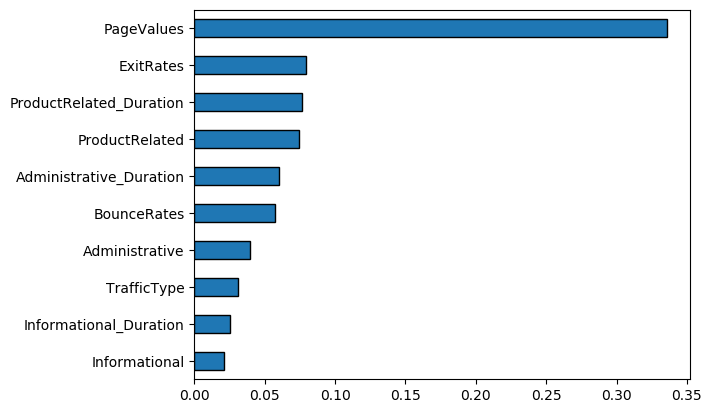
\includegraphics[width=8cm]{onlineshop/plots/feature_selection_random_forest_classifier.png}}

\capbtabbox{%
  \begin{tabular}{l|r}
Atribute                  & \multicolumn{1}{l}{Score} \\ \hline
ProductRelated\_Duration  & 877404.34                 \\
PageValues                & 175126.81                 \\
Administrative\_Duration  & 41754.84                  \\
Informational\_Duration   & 35059.78                  \\
ProductRelated            & 19317.29                  \\
Administrative            & 1133.97                   \\
Informational             & 357.98                    \\
Month\_Nov                & 223.55                    \\
VisitorType\_New\_Visitor & 115.34                    \\
Month\_May                & 55.00                     \\
SpecialDay                & 53.80                     \\
OperatingSystems\_3       & 48.55                    
\end{tabular}
}{%
  \caption{Top 10 features selected by SelectKBest}\label{tab:feat_sel}
}
\end{floatrow}
\end{figure}
Looking at both models, one can see that the two most important attributes are 'ProductRelated\_Duration' and 'PageValues.
Using the information from the two selections and through trial and error, by playing around with a few different attribute combinations, we have found the following top attributes:

\begin{itemize}
    \item Top 3: ['ProductRelated\_Duration', 'PageValues', 'Administrative\_Duration']
    \item Top 7: Top 3 + ['Informational\_Duration',  'ProductRelated', 'Administrative', 'Informational']
    \item Top 12: Top 7 +  ['BounceRates', 'ExitRates', 'PageValues', 'Month\_Nov', 'TrafficType' ]      
\end{itemize}
Performance comparisons between the different Top attributes lists can be found in the following sections.  



\subsection{K Nearest Neighbours Classifier}
Looking at \secref{fig:knn_wo_pre} one can see that using the most attributes leads to the best performance which holds true for the other Classifiers as well. Interesting to note here, is that the best recall values were achieved when using k = 1 and thus only looking at the closest neighbour. 

\begin{figure}
\begin{floatrow}
\ffigbox[\FBwidth][][]{\caption{Without Scaling (metric: Manhattan, weights: Uniform)}}
    {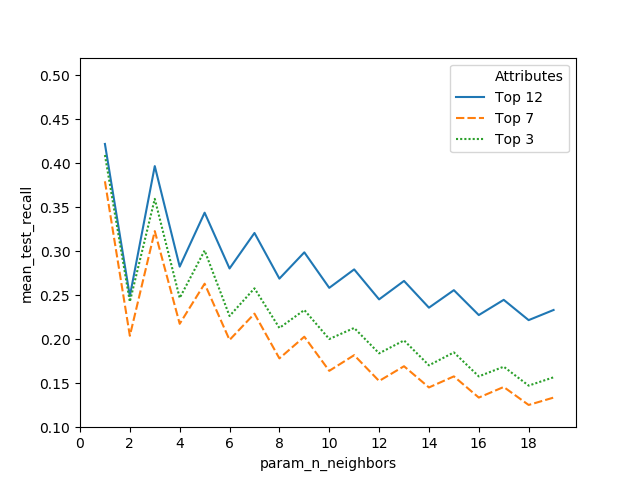
\includegraphics[width=6cm]{onlineshop/plots/knn_wo_preprocessing.png}\label{fig:knn_wo_pre}}
\ffigbox[\FBwidth][][]{\caption{With MinMax Scaling (metric: Uniform, Top 12 Attributes)}}
    {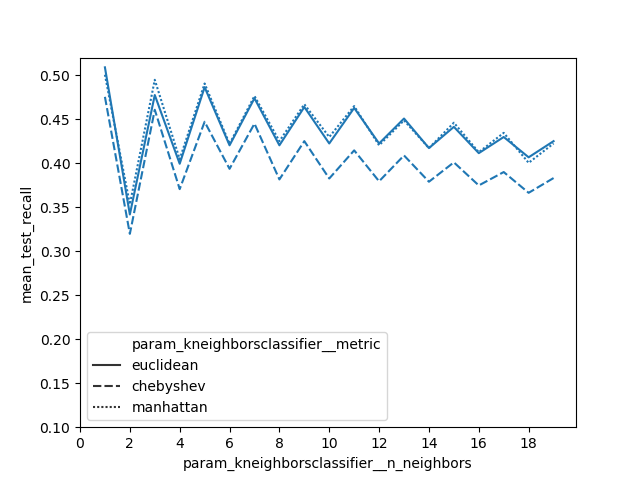
\includegraphics[width=6cm]{onlineshop/plots/knn_uniform_metric_comparison.png}\label{fig:knn_w_pre}}
\end{floatrow}
\end{figure}
A general analysis beforehand showed that, while different weight parameters change how the recall values react to different k's, with \textit{uniform} being more sensitive compared to  \textit{distance}, they do not change the best achievable values.\\
\newline
As can be seen in \secref{fig:knn_w_pre} scaling the data leads to a best case improvement of around 0.07 compared to the unscaled data. This effect increases with increasing k. Another thing that scaling the data does, is reducing the overall decrease of the recall with changing k. This figure also shows that the euclidean and manhattan metric perform very similar for this dataset while the chebyshev performs slightly worse. 

\subsection{Random Forest Classifier}
For Random Forest Classifier we have used GridSearchCV to try out a few different parameters like \textit{n\_estimators, max\_depth and the criterion}. \\
\newline
By doing a few pre tests and comparing how the criterion affects the recall value, we note that they lead to very similar results for this dataset. Since Gini is a tiny bit better than Entropy, it will be used for the other comparisons. \\
\newline

\begin{figure}
\begin{floatrow}
\ffigbox[\FBwidth][][]{\caption{Comparison of \textit{n\_estimators} for different \textit{max\_depth} values}}
    {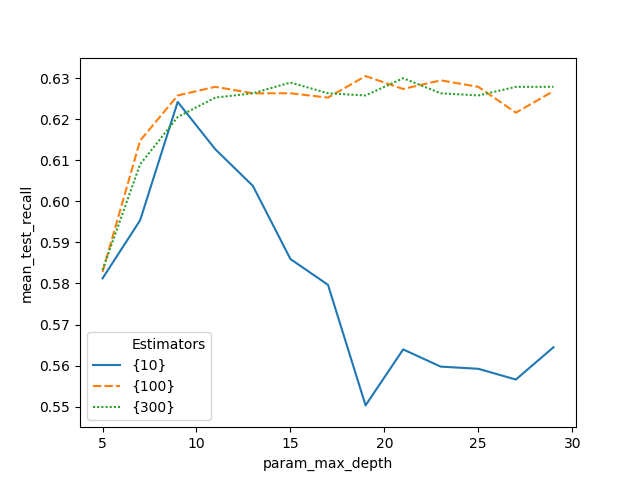
\includegraphics[width=6cm]{onlineshop/plots/rfc_n_estimators_comparison.png}\label{fig:rf_n_estim}}
\ffigbox[\FBwidth][][]{\caption{Scaling vs No Scaling comparison (100 Trees)}}
    {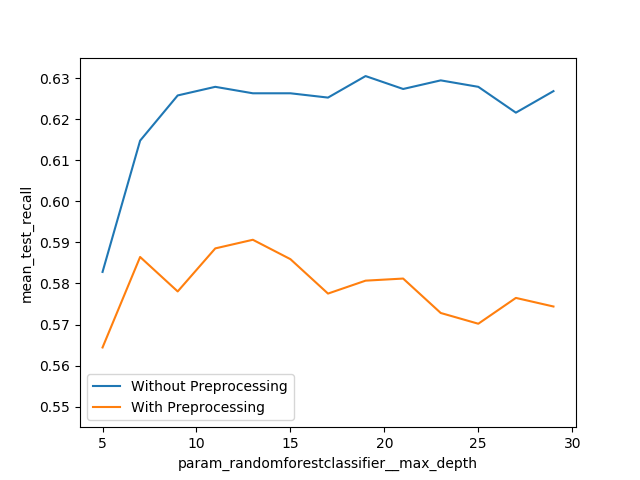
\includegraphics[width=6cm]{onlineshop/plots/rfc_preprocessing_comparison.png}\label{fig:rfc_pre}}
\end{floatrow}
\end{figure}
Looking at the different n\_estimators in \secref{fig:rf_n_estim} we can see that a higher n\_estimators makes up for the overfitting which will be achieved by having a too high max\_depth value. This makes sense as the amount of trees within a forest is a good way to control overfitting. On the other hand after a certain point it makes no difference if there are 100 or 300 trees. \\
\newline
As trees are very robust and thus do not need Preprocessing most of the time, applying a MinMaxScaler to our data actually led to worse values which is visualized in \secref{fig:rfc_pre}.

\subsection{Multi-Layer Perceptron Classifier}
Finally, taking a look at the more sophisticated Multi-Layer Perceptron, we have tried out a few different parameter settings, firstly manually configuring them and then iterating over a few different combinations with GridSearch. The paremeters we have looked at were: hidden layer sizes (layer and neuron amount), activation functions, different solvers, learning rate and the alpha penalty regularization parameter.


\begin{figure}
\begin{floatrow}
\ffigbox[\FBwidth][][]{\caption{Comparison of different \textit{hidden\_layer\_sizes} with stochastic gradient descent optimizer}}
    {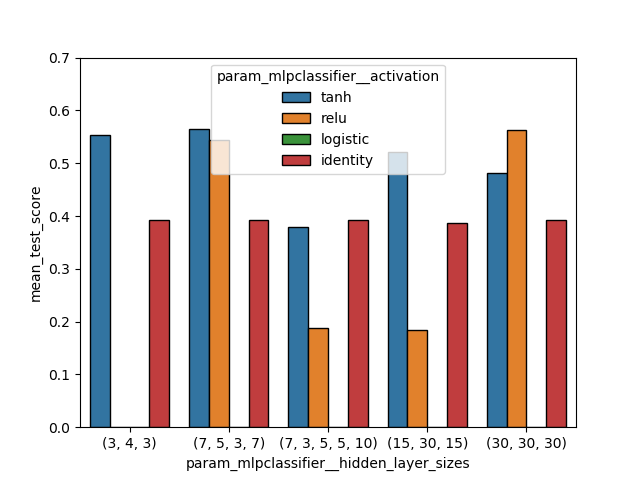
\includegraphics[width=6cm]{onlineshop/plots/mlp_solver_comparisonsgd.png}\label{fig:mlp_sgd}}
\ffigbox[\FBwidth][][]{\caption{Comparison of different \textit{hidden\_layer\_sizes} with adam optimizer}}
    {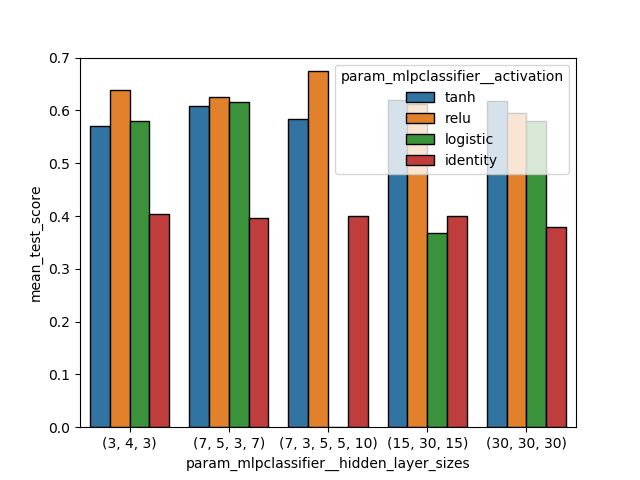
\includegraphics[width=6cm]{onlineshop/plots/mlp_solver_comparisonadam.png}\label{fig:mlp_adam}}
\end{floatrow}
\end{figure}
As can be seen in \secref{fig:mlp_sgd}, using the wrong weight optimizer (stochastic gradient descent in this case) leads to much worse recall scores, with some of them even being zero (no True Positives predicted). Using the stochastic gradient descent version adam (by Kingma, Diederik, and Jimmy Ba) we were able to achieve much better and more consistent scores.\\
\newline
On the other hand the difference between having a constant learning rate of 0.001 and an adaptive one (divide learning rate by 5 if the training loss does not decrease for 2 consecutive epochs) was negligible, with the adaptive one being only 0.02 better in the best case. The same goes for different alpha values. \\
\newline
What can be observed is that using tangens hyperbolicus and Relu provides far better results no matter the layer sizes. The identity function performed much worse, achieving only a recall score of around 0.4 while the others were able to achieve scores of above 0.6 for at least one parameter setting. On the other hand, while the logistic activation function even was able to achieve a better score than the tangens hyperbolicus (hidden layer sizes (3,4,3)), it performed much worse in a few settings (hidden layer sizes (7, 3, 5, 5, 10) or (15, 30, 15)) whereas the others stayed consistent. \\
\newline
It can be said, that while the hidden layer sizes obviously matter, the activation function played a much bigger role for getting the best values. On average for this dataset relu performed the best, followed by tangens hyperbolicus with logistic and identity performing the worst. The best result (0.6750 recall) was achieved when using more layers and relu as the activation function. The amount of neurons seemed to not make too much of a difference.


\subsection{Conclusion}
\subsubsection{Preprocessing vs No-Preprocessing}
To be able to look at more than just the numerical values, \textit{No-Preprocessing} in this case stands for the data after the general Preprocessing (One Hot Encoding, remove Missing values, ...), mentioned in \secref{GenPrepro}, has been done. We compare the unpreprocessed data with the data after MinMax scaling.\\% and after introducing a new feature by weighting the outliers.
\newline
Analysing \secref{tab:onl_pre_no_pre}, we can see that using a MinMax Scalar only works for the K Nearest Neighbors Classifier and the Multi-Layer Perceptron. As the Random Forest Classifier does not work with distances,  the ranges of the different attributes does not matter. Hence using a MinMaxScaler actually leads to worse results for the Random Forest Classifier.

% TODO

\begin{table}[h]
\begin{center}
\begin{tabular}{|l|l|l|}
\hline
                       & Preprocessing & No-Preprocessing \\ \hline
KNeighborsClassifier   & \textbf{0.5089}        & 0.4219          \\ \hline
RandomForestClassifier & 0.5906        & \textbf{0.6305}           \\ \hline
MLPClassifier          & \textbf{0.6750}        & 0.6106           \\ \hline
\end{tabular}
\caption{Recall comparison with- and without MinMax Scaling}
\label{tab:onl_pre_no_pre}
\end{center}
\end{table}

\subsubsection{Holdout vs Cross Validation}
The cross validation results are the best ones achieved during the GridSearch parameter iteration, hence they are the same ones as the ones as in the table of the previous section (Preprocessing values for KNeighborsClassifier and MLPClassifier, No-Preprocessing for RandomForestClassifier). To calculate the Holdout score we used the best parameters of the respective Classifier and then fit the data on that estimator. 
By comparing the achieved holdout and cross validation values we can see that the holdout method sometimes leads to better results and sometimes to worse. This is a possibility since the training split is randomly chosen, which plays a big part in how the data will be tested. In these particular cases Holdout led to only marginally better results for KNeighborsClassifier and RandomForestClassifier, while MLPClassifier was surprisingly a lot better while using Cross Validation. 

\begin{table}[h]
\begin{center}
\begin{tabular}{|l|l|l|}
\hline
                       & Holdout & Cross Validation \\ \hline
KNeighborsClassifier   & \textbf{0.5236}  & 0.5089           \\ \hline
RandomForestClassifier & \textbf{0.5863}  & 0.5817           \\ \hline
MLPClassifier          & 0.5681  & \textbf{0.6750}           \\ \hline
\end{tabular}
\caption{Comparison of accuracy of holdout versus cross-validation}
\end{center}
\end{table}

%
\subsubsection{Different Performance Metrics}
To analyse how the different classifiers compare for this dataset we have tried to optimize the models in regards to recall as mentioned above. Using GridSearchCV's best\_estimator we were able to find the optimal parameter settings, which were as follows (if parameters are undefined, the default ones for the respective sklearn models were chosen):
\begin{itemize}
    \item K Neigbors Classifier: MinMax Scaling, leaf\_size=30, n\_neighbors=1, metric='euclidean', 
    \item Random Forest Classifier: No Scaling, criterion='gini', max\_depth=19, max\_features='auto', n\_estimators=100
    \item MLP Classifier: MinMax Scaling, activation='relu', alpha=0.001,\\learning\_rate='adaptive',
    learning\_rate\_init=0.001, max\_iter=3000, \\ hidden\_layer\_sizes=(7, 3, 5, 5, 10) (some parameters may change due to randomness)
\end{itemize}

\begin{table}[h]
\begin{center}
\begin{tabular}{|l|l|l|l|l|l|}
\hline
                       & Accuracy & Precision & Recall & F1     & Runtime (sec) \\ \hline
KNeighborsClassifier   & 0.8525   & 0.5483  & 0.5089 & 0.5213 & \textbf{0.0434}        \\ \hline
RandomForestClassifier & \textbf{0.8982}   &\textbf{0.7187}    & 0.5817   & \textbf{0.6408}   & 1.0573        \\ \hline
MLPClassifier          & 0.8914   & 0.6648    & \textbf{0.6152}   & 0.6375   & 5.3267        \\ \hline
\end{tabular}
\caption{Comparison of different performance metrics and runtimes}
\label{tab:onl_summ}
\end{center}
\end{table}

Analysing the table in regards to Accuracy, we see that the different classifiers all perform very similarly, with K Neighbors Classifier being around 4 percent worse than the others. This is to be expected since our data is quite skewed, only having around 15.5\% positive target values. Due to this it is especially important to look at the other performance metrics. \\
\newline
While RandomForest Classifier only is marginally better than MLP Classifier in regards to accuracy, it achieves a precision score of around 72 percent which is more than 5 percent better than the one achieved by MLP and more than 5 percent better than the one achieved by K Neighbors. \\
\newline 
Using GridSearchCV to optimize our model in regards to recall, we were able to achieve a recall score of around 62 percent with the MLP Classifier and a score of 58 percent with the Random Forest Classifier. Looking at the F1 score we can see that Random Forest Classifier and MLP Classifier perform very similarly, both achieving a worthy score of around 0.64.\\
\newline
Concering runtime we can see that the K Neighbors Classifier obviously performs best as it is a lazy learner and does not need any pre fitting. With increasing complexity, the runtime also increases which is why the MLP Classifier took over a hundred times longer to fit than the K Neighbors Classifier and over 5 times longer than the Random Forest Classifier.\\
\newline
To answer the question, which Classifier performs best for this dataset, we need to differentiate a few different scenarios.
If we only care about the accuracy score and need to get results fast, the best option would be the K Neighbors Classifier as it performs a lot better in regards to runtime and is comparable in terms of accuracy.\\
Comparing the Random Forest Classifier and the MLP Classifier we can see that there is a draw in terms of Accuracy and F1 since the differences between the two classifiers are negligible. If we say that a high precision, i.e. there is a higher cost of falsely identifying Positives, and a faster runtime are more important, then the Random Forest Classifier would be the best choice.\\
Since we defined that recall is our most important metric (the opportunity costs of passing up on a buying candidate are high) the MLP Classifier is the best one for this particular dataset.
\newpage

